\documentclass[12pt]{report}
\usepackage[T1]{fontenc}
\usepackage[french]{babel}
\usepackage[utf8x]{inputenc}
\usepackage{amsmath}
\usepackage{graphicx}
\usepackage[colorinlistoftodos]{todonotes}

\begin{document}



%-----------------------------------------------------------------%
%    PAGE DE TITRE
%-----------------------------------------------------------------%

\begin{titlepage}

\newcommand{\HRule}{\rule{\linewidth}{0.7mm}} % Trait horizontal

\center
 
%---------------------------%
%   LOGO & EN-TÊTE DE PAGE
%---------------------------%

\includegraphics[width=0.8\textwidth]{img/logo.jpg}\\

\textsc{\Large Projet de Programmation}\\[0.5cm]
\textsc{\large Génération procédurale de planètes}\\[0.5cm]

%---------------------------%
%   TITRE
%---------------------------%

\HRule \\[0.4cm]
{ \huge \bfseries Cahier des besoins}\\[0.4cm]
\HRule \\[1.5cm]
 
%---------------------------%
%   AUTHEURS
%---------------------------%

\begin{minipage}{0.4\textwidth}
\begin{flushleft} \large
\emph{Auteurs:}\\
Rémy \textsc{Maugey}\\
Jérémi \textsc{Bernard}\\
Hugo \textsc{Alonso}\\
Brian \textsc{Mazé}\\
\end{flushleft}
\end{minipage}
~
\begin{minipage}{0.4\textwidth}
\begin{flushright} \large
\emph{Client:} \\
Emmanuel \textsc{Fleury}
\end{flushright}
~
\begin{flushright} \large
\emph{Chargé de TD:} \\
Boris \textsc{Mansencal}
\end{flushright}
\end{minipage}\\[2cm]

%---------------------------%
%   DATE
%---------------------------%

{\large 22 Janvier 2018}\\[2cm] 


\vfill % Fill the rest of the page with whitespace

\end{titlepage}
%-----------------------------------------------------------------%
%   FIN PAGE DE TITRE
%-----------------------------------------------------------------%

%-----------------------------------------------------------------%
%   Table des Matières
%-----------------------------------------------------------------%


\tableofcontents

\thispagestyle{empty} % empeche l'affichage du numero de cet page

%-----------------------------------------------------------------%
%   Introduction
%-----------------------------------------------------------------%

\newpage

\chapter*{Introduction}
\addcontentsline{toc}{chapter}{Introduction}
\setcounter{chapter}{1}

Un objet en trois dimensions complexe est un ensemble de sommets reliés
entre eux par des arrêtes, formant des faces triangulaires. L'ensemble
de ces points et arrêtes est appelé maillage. Ces triangles sont ensuite
traités et affichés à l'écran en deux dimensions. Plus le nombre de
triangles à afficher est élevé, plus le rendu d'une image est long, ce
qui est problématique dans une application nécessitant de générer
beaucoup d'images rapidement, par exemple pour un rendu temps réel dans
une simulation ou un jeu vidéo.\\
Il est alors intéressant de pouvoir réduire le nombre de triangles d'un
objet qui n'a pas besoin d'être très détaillé dans un cas précis, par
exemple si l'objet est loin de l'observateur. Un cas particulier est
l'affichage d'une surface très grande comportant des aspérités, par
exemple un terrain. Une partie du terrain est proche de l'observateur,
nous voulons donc en afficher les détails, mais une autre partie est
plus éloignée, et les détails seront moins visibles sur l'image finale.
On peut donc réduire le nombre de triangle de la partie éloignée afin de
réduire le nombre de triangles à traiter.

L'objectif de ce projet est d'implémenter un système de \emph{LOD} (
\emph{Level of Detail}: niveau de détail) à appliquer sur le maillage
d'une sphère en vue d'une application en temps réel, afin d'optimiser
son affichage. Le projet comportera aussi une application permettant le
rendu de cette sphère en trois dimensions, afin de pouvoir visualiser le
fonctionnement du système de \emph{LOD}, ainsi qu'un moyen de mesurer
les performances du système. Comme demandé, notre projet se basera sur
la méthode proposée dans \cite{CDLOD}, permettant de générer le
maillage en temps réel en fonction de la distance à la caméra. Nous
adapterons la méthode de \cite{CDLOD} qui utilise le \emph{GPU}
pour développer une version \emph{CPU}. Cette méthode a l'avantage de
rattacher les maillages des différents niveau de détail de manière lisse
et progressive, c'est à dire sans frontières intermédiaires, rendant le
résultat homogène. Un autre avantage de cette méthode est de garder le
nombre de triangles affichés constant, en répartissant les triangles
dans les différents niveaux de détails.

%-----------------------------------------------------------------%
%   État de l’existant
%-----------------------------------------------------------------%
\newpage

\chapter*{État de l'existant}
\addcontentsline{toc}{chapter}{État de l'existant}
\setcounter{chapter}{2}

L'objectif final du projet est d'optimiser l'affichage de la planète grâce à un système de niveau de détails variant en fonction de l'éloignement de la caméra. Plusieurs implémentations allant dans ce sens existent et ont déja été publiées.
Notre projet sera basé sur la technique décrite par Filip Strugar en 2010, \textit{Continuous Distance Dependent Level of Detail for Rendering Heightmaps}.
D'autre projets similaires existent mais utilisent des structures de données différentes, l'utilisation d'un système de \textbf{chunks} ou encore de \textbf{clipmaps}. Bien que toutes ces techniques soient différentes, elles se basent sur le même principe fondamental, rajouter à la volée des détails sur les objets proches.


%http://tulrich.com/geekstuff/sig-notes.pdf
%http://hhoppe.com/gpugcm.pdf
%http://dept-info.labri.fr/~narbel/PdP/Subjects17-18/Papers/cdlod_latest.pdf

%-----------------------------------------------------------------%
%   ANALYSE DES BESOINS
%-----------------------------------------------------------------%
\newpage

\chapter*{Analyse des besoins}
\addcontentsline{toc}{chapter}{Analyse des besoins}
\setcounter{chapter}{3}

%% Trier les besoins :

% Créer une structure de données quadtree
% Stocker des heightmaps dans les quadtree
% Générer des heightmaps
% Crééer une lib pour gérer les quadtrees (voir ça comme une base de données) => demande(theta, rho) => DB => return z;
% Convertir les coordonnées x,y de la heightmap en coordonnées polaires
	% x = rho cos theta
    % y = rho sin theta

% Récupérer la hauteur z dans le quadtree
% Faire une sphère avec un maillage hiérarchique
% Afficher la sphère avec opengl
% Paramètre de l'application : -d Density -i Init point
% Faire les tests unitaires // pourquoi (hugo)? L'appli a pas besoin d’être robuste. Les test unitaires seront durs à implémentés
% Test de performance (en fonction de la densité)
% Afficher un compteur de fps
% Densité changeable en live (par ex avec + et -), peut être afficher aussi la densité
% Doc et commentaire en anglais
% CI avec travis, style de codage cohérent
% Utilisation de triangle pour représenter le maillage

% Se déplacer dans la scène 3d
%Gérer les événements clavier et souris. Les mettre en relation avec une classe caméra. Prendre en compte cette caméra dans la boucle d'affichage de la sphère afin de pouvoir se déplacer dans la scène 3D.

%---------------------------%
%   BESOINS FONCTIONNELS
%---------------------------%

\section{Besoins fonctionnels}

\subsection{Génération de terrain}

Générer la carte de hauteur d'un terrain.\\
Construire une sphère à partir de la carte rectangulaire afin d'obtenir
une planète.


\subsection{Interface graphique}



\subsection{Interface graphique}

Générer une carte de hauteur décrivant le terrain de la planète, et l'utiliser pour former le maillage d'une sphère et l'afficher à l'écran. L'utilisateur doit pouvoir déplacer la caméra en trois dimensions dans la scène à l'aide du clavier et/ou de la souris.

\subsection{Structure de donnée}

Implémenter une structure de donnée représentant un quad-tree à utiliser avec les algorithmes de CDLOD (voir figure \ref{fig:quadtree})

\begin{figure}[!ht]
  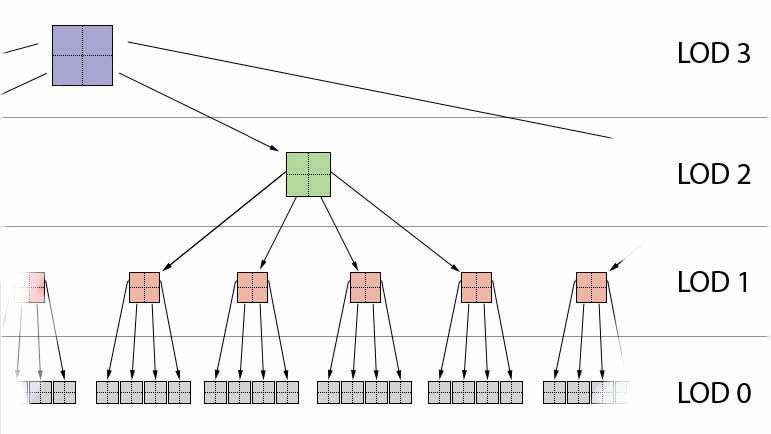
\includegraphics[scale=0.5]{img/Quadtree.png}
  \caption{Quad-tree}
  \label{fig:quadtree}
\end{figure}

\subsection{CDLOD}

Implémenter un algorithme de CDLOD permettant de générer des niveaux de détails d'une carte de hauteur. L'algorithme doit être implémenté sous forme de quadtree, et livré dans une bibliothèque séparée du programme principal. La bibliothèque fonctionne comme une base de données. Les paramètres des requêtes sont le niveau de détail demandé (le niveau de détail le plus bas correspond à la carte de hauteur d'origine) et la zone ou le point demandé, sous forme de coordonnées polaires. La base de donnée converti ces coordonnées polaires en coordonnées sur le plan de la carte de hauteur.

Associer la bibliothèque de niveau de détail avec l'affichage de la scène. Le maillage de la planète doit s'adapter à la distance à la caméra. Plus la caméra est éloignée d'un point, moins ce point doit être détaillé (son niveau de détail est plus grand).

\subsection{Mesure des performances}

Afficher le nombre de trames par seconde à l'écran.

Proposer un moyen de mesurer les performances à l’exécution (temps nécessaire pour générer une image, réponse de la base de données, ...).
% J'aime pas cette phrase et c'est moi qui l'ai écrite -Rémy


\subsection{Documentations}

Documenter les interfaces du projets ainsi que les implémentations, en anglais. La documentation des interfaces doit être extractible.
% Je veux vraiment sortir doxygen pour le principe, mais on peut faire sauter le passage dans les besoins. -Rémy
Utiliser un style de code défini.


\subsection{Tests}

Mettre en place des tests unitaires. Tout les tests  seront utilisés au long du projet afin de vérifier que les nouvelles fonctionnalités apportées ne dérangent pas le bon fonctionnement des précédentes.
% ctest pour les tests ? C'est livré avec CMake donc pas chiant pour les lancer.
% D'intégration ? De validation ? Ca commence à faire beaucoup de tests mais ça peut être intéressant les tests d'intégration -Rémy


%---------------------------%
%   BESOINS NON-FONCTIONNELS
%---------------------------%
\newpage

\section{Besoins non-fonctionnels}
\subsection{Intégration continue}

Mettre en place un système d'intégration continue en parallèle au projet afin d'éxécuter les tests et de formater le code de manière uniforme.
% A appliquer avec un outil type clang-format. Va falloir le définir
% A chacun de configurer son git pour lancer l'outil avant chaque commit -Rémy


\subsection{Gestionnaire de versions }
Utiliser un outil de gestion de version afin de disposer d'un dépôt partagé et de suivre l'évolution du projet. Git sera l'outil utilisé, avec un dépôt hébergé sur le serveur Savane du CREMI.

%-----------------------------------------------------------------%
%   MISE EN OEUVRE
%-----------------------------------------------------------------%
\newpage

\chapter*{Mise en Oeuvre}
\addcontentsline{toc}{chapter}{Mise en Oeuvre}
\setcounter{chapter}{4}



%---------------------------%
%   DIAGRAMME DE GRANT
%---------------------------%

\section{Diagramme de Gantt}


%TODO 

\bibliography{biblio}{}
\bibliographystyle{plainnat}


\end{document}
